\RequirePackage[T1]{fontenc}
\documentclass[conference]{IEEEtran}
\usepackage{cite}
\usepackage{graphicx}
\usepackage{amsmath,amssymb,amsfonts}
\usepackage{textcomp}
\usepackage[hyphens]{url}
\usepackage{array}
\usepackage[hidelinks]{hyperref}
\usepackage{xcolor}
\emergencystretch=3em
\setcounter{dbltopnumber}{2}
\renewcommand{\dbltopfraction}{0.95}
\renewcommand{\dblfloatpagefraction}{0.85}
\renewcommand{\textfraction}{0.05}
\newcommand{\CADDAM}{CADD\allowbreak{}+\allowbreak{}AlphaMissense}
\newcommand{\GCNCADDAM}{GCN\allowbreak{}+\allowbreak{}CADD\allowbreak{}+\allowbreak{}AlphaMissense}

\title{Auditing PPI Graph Augmentation for Missense Variant Pathogenicity Prediction under Topology, Connectivity and Homology Constraints}

\author{\IEEEauthorblockN{Yuxin Tian, Xianguo Zhang\textsuperscript{*}, Weibo Meng, Jieqi Yin, and Yongqin Jin}
\IEEEauthorblockA{College of Computer Science (College of Software), College of Artificial Intelligence\\
Inner Mongolia University, Hohhot 010021, China\\
Email: yuxin\_t02@163.com; 2595083628@qq.com\\
\textsuperscript{*}Corresponding author: Xianguo Zhang}}
\hypersetup{pdfauthor={Yuxin Tian, Xianguo Zhang, Weibo Meng, Jieqi Yin, Yongqin Jin}}

\begin{document}
\maketitle
\raggedbottom


\begin{abstract}
\bfseries\boldmath
Protein-protein interaction (PPI) graphs can add molecular context to missense variant prediction, but their contribution depends on evaluation design and baseline strength. We audit fixed two-hop propagation of ESM protein embeddings using 177,213 ClinVar variants and a STRING association graph. Only downstream classifiers are trained. Across three seeds, propagation increased mean AUC from 0.7835 to 0.7950; protein-clustered intervals for the reference-model gains included zero. Connectivity and topology controls showed performance sensitivity, although their propagation and training settings were not fully matched. With CADD and AlphaMissense included, protein-representation controls retained much of the fusion gain. Under homology-aware splitting, the single graph-fusion estimate was below the repeated strong-predictor baseline. Exploratory analyses described variation across topology groups and prediction-error transitions. BioGRID second-network validation did not establish a consistent added benefit over raw-embedding controls. These findings support context-dependent protein-representation complementarity and careful evaluation of network-specific increments. They concern fixed propagation and should not be generalized to trained graph neural networks.

\end{abstract}

\begin{IEEEkeywords}
\bfseries\boldmath
Missense variant pathogenicity, protein-protein interaction networks, graph augmentation, protein language models, homology-aware evaluation.
\end{IEEEkeywords}

\section{Introduction}

Missense variant pathogenicity prediction has been advanced by established methods such as CADD, REVEL, MVP, PrimateAI, EVE and AlphaMissense \cite{Kircher2014CADD,Ioannidis2016REVEL,Qi2021MVP,Sundaram2018PrimateAI,Frazer2021EVE,Cheng2023AlphaMissense}, as well as by protein language models such as ESM \cite{Lin2023ESM}. These approaches capture sequence, evolutionary and annotation-derived signals. Disease-associated proteins are also embedded in molecular interaction networks, and disease-associated mutations can perturb protein-protein and other macromolecular interactions \cite{Barabasi2011NetworkMedicine,Menche2015DiseaseModules,Sahni2015InteractionPerturbation,Chen2018InteractomePerturbation}. PPI graphs provide an additional source of context for missense variant prediction.

Earlier approaches incorporated protein-interaction and other molecular-network features into single-amino-acid variant prioritization, showing that network context can provide information complementary to sequence, structure and annotation features \cite{Yates2014SuSPect,Ozturk2022NetworkFeatures}. More recent graph-based variant predictors include graph attention models for missense effects, heterogeneous gene-variant graph approaches, multimodal variant graph methods and disease-specific graph models \cite{Zhang2022gMVP,Cheng2021VEGN,Yu2025GNNMAP,Ghadie2025DiseaseSpecificGNN}. These studies establish the relevance of relational structure to variant interpretation. We focus on how to interpret gains obtained by propagating protein language model embeddings over a shared STRING PPI graph before variant-level classification.

A shared-graph setting mixes several effects. Train, validation and test variants may have distinct protein identifiers while their proteins remain directly connected in the same PPI graph. Related proteins may also cross partitions when homology is not explicitly controlled \cite{Littmann2022ProteinMLTips,Teufel2023GraphPart}. Strong variant-effect predictors such as CADD and AlphaMissense can further reduce the marginal contribution of graph propagation. We evaluate protein-topology correspondence, graph connectivity, protein-level uncertainty, homology-aware performance and complementarity to established predictors.

We conduct a systematic audit using a reconstructed ClinVar-STRING missense dataset and evaluate raw ESM representations, fixed PPI-GCN propagation, CADD, AlphaMissense and fusion models. The study makes three contributions. First, it provides an evaluation framework that examines graph topology, representation complementarity, train-test graph connectivity and downstream classifier configuration. Second, it quantifies how strong variant-effect predictors and homology-aware splitting change the apparent value of PPI graph augmentation. Third, it relates graph-associated gains and prediction changes to topology contexts and error transitions through exploratory analyses. A second-network evaluation using BioGRID tests the dependence of the findings on network choice.

\section{Materials and Methods}

\subsection{Dataset and graph construction}

ClinVar variant annotations were obtained from the official NCBI ClinVar FTP tab-delimited variant-summary file \cite{Landrum2020ClinVar}. Checksums and sample identifiers freeze the processed benchmark; its exact ClinVar content-release date could not be verified. We reconstructed a filtered, non-conflicting missense dataset and mapped variants to STRING human protein identifiers. We retained GRCh38 germline missense SNVs with criteria-supported review status, combined pathogenic and likely pathogenic records into the positive class, combined benign and likely benign records into the negative class, removed uncertain or conflicting records, and collapsed duplicate VariationIDs. The final ClinVar-STRING dataset contained 177,213 missense variants mapped to 14,123 labelled STRING proteins. The propagation graph contained 19,622 STRING protein nodes and 13,715,404 directed edge-index entries from the STRING v12 protein-association network \cite{Szklarczyk2023STRING}. We used this network as PPI context; its association evidence extends beyond direct physical interactions.

\subsection{Protein representations and PPI propagation}

Raw protein features were generated using the ESM-2 650M checkpoint, with 1,280-dimensional protein-level vectors obtained by residue averaging \cite{Lin2023ESM}. PPI-GCN embeddings were computed by fixed two-hop GCN-style propagation over the normalized STRING graph \cite{Kipf2017GCN}. We use ``PPI-GCN'' as shorthand for fixed GCN-style propagation of ESM features; no graph-convolution parameters were learned. Fixed propagation isolates topology-induced smoothing from capacity gains due to trainable graph layers and provides a controlled representation for the audit. Let $X$ denote the raw ESM protein-representation matrix. The full-graph implementation added self-loops before symmetrization and summed duplicate entries, giving two self-loop contributions. Let $\tilde{A}$ denote this weighted adjacency matrix and $\tilde{D}$ its degree matrix. We computed the symmetrically normalized adjacency matrix as
\begin{equation}
\hat{A}=\tilde{D}^{-\frac{1}{2}}\tilde{A}\tilde{D}^{-\frac{1}{2}},
\end{equation}
\begin{equation}
H=\frac{1}{3}\left(X+\hat{A}X+\hat{A}^{2}X\right).
\end{equation}
The fixed two-hop PPI-GCN representation $H$ averages the original ESM features, one-hop PPI-smoothed features and two-hop PPI-smoothed features. Propagation used only graph structure and ESM features; downstream classification used the representation of each variant's mapped STRING protein. The full graph contained train, validation and test nodes with their ESM features, making the evaluation transductive. Protein-only inputs cannot distinguish variants within the same protein.

\subsection{Splits, classifiers and external predictors}

The original split assigned train, validation and test variants by STRING protein ID, with no shared proteins across partitions. The split contained 141,864 training variants, 17,129 validation variants and 18,220 test variants. The homology-aware split used MMseqs-derived protein clusters, assigned each cluster wholly to one partition and preserved the same row counts \cite{Steinegger2017MMseqs2}. We use this split as a stress test. Its test positive rate was 10.56\%, compared with 31.95\% in the original split, which limits direct cross-split AUPRC comparison.

All representation and fusion models were evaluated with a downstream MLP classifier selected by validation AUC and optimized with Adam \cite{Kingma2015Adam}. Multi-feature representation and fusion models used a 512/128 hidden-layer MLP with dropout 0.3. Low-dimensional external-score baselines used a smaller 32/16 classifier with dropout 0.2. Architecture-matched \CADDAM{} and fusion-control comparisons used the same 512/128 hidden-layer architecture and preprocessing, with different input-layer parameter counts. Training used mini-batches of 1,024 variants, learning rate $10^{-3}$, weight decay $10^{-5}$, a maximum of 50 epochs (30 for the representation ablation/permutation controls) and early stopping after five consecutive validation checks without improvement in validation AUC. Class imbalance was handled with \texttt{BCEWithLogitsLoss} using training-partition positive-class weight $N_{\mathrm{negative}}/N_{\mathrm{positive}}$. CADD GRCh38 v1.7 scores and AlphaMissense hg38 scores were matched to the reconstructed variants \cite{Kircher2014CADD,Schubach2024CADDv17,Cheng2023AlphaMissense}. CADD scores covered 177,205 variants (99.995\%), and AlphaMissense scores covered 171,753 variants (96.92\%). Missing CADD and AlphaMissense scores were imputed with training-set medians; AlphaMissense-based feature sets also included a binary missingness indicator. In the evaluated MLP configurations, no additional z-score standardization was applied to CADD, AlphaMissense or embedding-derived inputs. All architecture-matched fusion controls shared the same preprocessing and feature construction. Alternative feature-scaling strategies were not evaluated. Seeds and repeat counts varied by analysis (Table~\ref{tab:runs}; Supplementary Table 8).

\subsection{Audit analyses}

Uncertainty was assessed using variant-level bootstrap and protein-clustered bootstrap \cite{Efron1993Bootstrap}. Connectivity tests removed direct train-test PPI edges and regenerated PPI-GCN embeddings. Partial edge-ablation curves removed 0\%, 25\%, 50\%, 75\% and 100\% of direct train-test protein pairs using random removal, higher-STRING-score-first removal and lower-STRING-score-first removal. Topology permutation preserved the unlabeled graph structure and randomized the correspondence between protein identity and graph position, testing whether generic graph smoothing explained the gain. Fusion controls concatenated \CADDAM{} features with raw ESM, edge-ablated PPI-GCN and topology-permuted PPI-GCN representations. The ablated/permuted encoders added one self-loop after symmetrization, unlike the full encoder. These comparisons do not isolate topology from normalization and training differences.

Topology-context analyses stratified test variants by degree, k-core, betweenness, clustering coefficient, neighbour-risk and community-boundary features. Neighbour-risk and neighbour pathogenic-rate features for validation and test proteins were computed from training-set labels only; validation and test labels were not used to construct these topology-context features. Corrected-sample analyses compared variants whose predictions were corrected or degraded after adding graph context. Topology-feature profiles are descriptive: multiple variants share each protein's features, and false-discovery-rate correction \cite{Benjamini1995FDR} does not address this dependence. No inferential significance is claimed for these profiles. AUPRC was interpreted within each split because precision-recall metrics are sensitive to class prevalence \cite{Saito2015PrecisionRecall}.

\begin{table}[t]
\caption{Summary of fitted models and repeated runs.}
\label{tab:runs}
\centering
\footnotesize
\begin{tabular}{@{}p{0.43\columnwidth}p{0.51\columnwidth}@{}}
\hline
Analysis & Fits and configuration \\
\hline
Fig. 1B,C; Fig. 2D & One reference fit per model \\
Fig. 1D: edge ablation & Five ablated fits; 30 epochs \\
Fig. 1E: partial ablation & Three per interior setting; 30 epochs; endpoints reused \\
Fig. 1F: permutation & Three graphs $\times$ three seeds; 30 epochs \\
Fig. 2B,C: original fusion & Three per arm; nine for permutation \\
Fig. 2E: homology fusion & Scores/raw fusion: three; graph fusion: one \\
Figs. 3B--F and 4 & Fixed reference prediction pairs \\
BioGRID comparison & Three per setting; 50 epochs \\
\hline
\end{tabular}
\par\smallskip\raggedright\footnotesize
The text also reports three-seed raw/full representation means. Fig. 1D--F reuse single-fit raw/full references. Bootstrap resamples are not classifier fits. Complete seeds, budgets and SD definitions are in Supplementary Table 8.
\end{table}

\subsection{Second-network validation}

BioGRID 5.0.262 human physical interactions \cite{Stark2006BioGRID} were mapped to the same 19,622 nodes, yielding 931,458 undirected edges after excluding RNA-related methods and ambiguous mappings. Nine classifiers covered representations under the original split and score fusion under both splits. Within this comparison, BioGRID and STRING used the same full-graph propagation convention; all models shared seeds 42--44, validation selection and a 50-epoch budget with patience five. Predictions were aligned by variant and protein identifiers and averaged in float64. Paired protein-bootstrap 95\% intervals used 2,000 resamples conditional on fitted models, without retraining or multiplicity adjustment (Supplementary Methods 5 and Table 9).

\section{Results}

\subsection{Full-graph PPI-GCN and connectivity sensitivity}

Under the original protein-level split, a retained reference run used for paired graph-ablation and bootstrap analyses gave raw ESM test AUC 0.7790 and AUPRC 0.6074. PPI-GCN improved these values to AUC 0.7997 and AUPRC 0.6496, corresponding to $\Delta$ AUC = +0.0207 and $\Delta$ AUPRC = +0.0421 (Fig. 1B). Across three classifier seeds, mean metrics (population SD) showed a smaller positive AUC difference: raw ESM reached AUC 0.7835 $\pm$ 0.0051 and AUPRC 0.6116 $\pm$ 0.0054; PPI-GCN reached AUC 0.7950 $\pm$ 0.0013 and AUPRC 0.6484 $\pm$ 0.0096. Variant-level bootstrap of the retained reference run gave $\Delta$ AUC +0.0208, 95\% CI [0.0174, 0.0240], and $\Delta$ AUPRC +0.0420, 95\% CI [0.0353, 0.0484]. Protein-clustered bootstrap widened both intervals across zero: $\Delta$ AUC CI [-0.0080, +0.0527] and $\Delta$ AUPRC CI [-0.0021, +0.0798] (Fig. 1C).

The full graph contained 1,242,422 direct train-test edge-index entries, representing 9.06\% of all edge-index entries and 621,211 unique undirected train-test protein pairs. Removing all direct train-test PPI edges reduced edge-ablated ESM-GCN to AUC 0.7791 $\pm$ 0.0076 and AUPRC 0.6255 $\pm$ 0.0148 (Fig. 1D). Relative to the raw-ESM reference, these point differences were $\Delta$ AUC +0.0001 and $\Delta$ AUPRC +0.0181; they do not establish equivalence. Partial ablation showed that AUC gain declined as direct train-test pairs were removed, with higher-STRING-score edge removal generally causing stronger loss at intermediate and high removal fractions (Fig. 1E).

Topology permutation preserved graph structure and randomly reassigned protein identities to graph positions. The resulting ESM-GCN achieved AUC 0.7757 $\pm$ 0.0067 and AUPRC 0.6052 $\pm$ 0.0086, close to raw ESM and below real PPI-GCN (Fig. 1F). These sensitivity comparisons are descriptive because operator, seed and training-budget differences prevent attribution solely to topology or direct connectivity.

\begin{figure*}[!t]
\centering
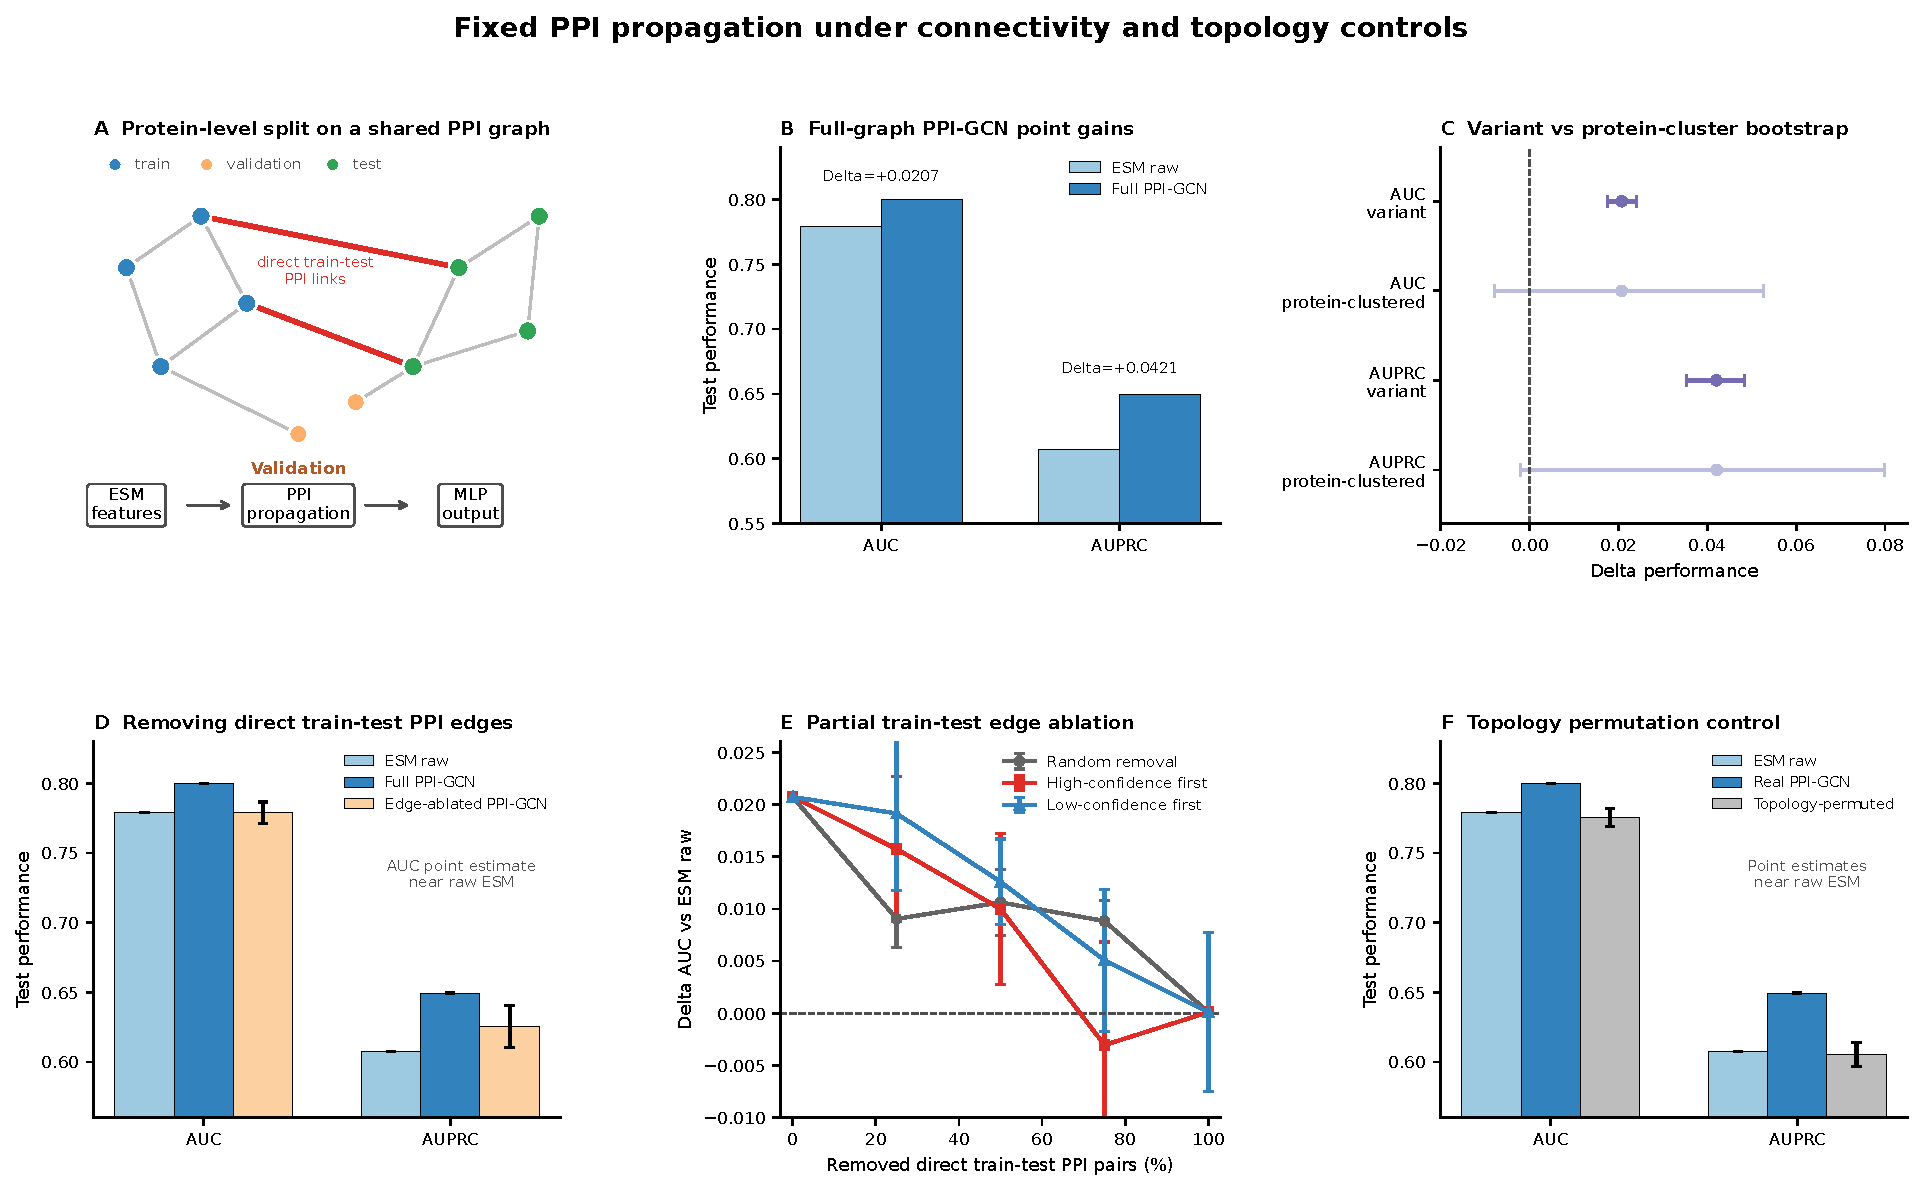
\includegraphics[width=0.98\textwidth]{figure_drafts/Figure1_connectivity_topology_controls_v2_accepted.pdf}
\caption{Workflow and primary audit of fixed PPI propagation. A, Audit design. B, Single-fit raw/full reference comparison; three-seed means are reported in the text. C, Paired differences with variant-level and protein-clustered bootstrap 95\% intervals; definitions are in Supplementary Table 4A. D, Direct train-test edge ablation. E, Partial ablation with three fits per interior setting, a single-fit full endpoint and a five-fit ablated endpoint. F, Topology permutation. D and F compare five ablated and nine permuted fits with single-fit raw/full references. Error bars show sample SD where repeated fits exist; permutation SD pools graph and classifier variation. Operator and training differences limit causal interpretation of these controls.}
\label{fig:connectivity}
\end{figure*}

\subsection{Strong predictors and homology-aware evaluation bound PPI context gains}

Under the original split, the external variant-effect predictors provided strong baselines. The single-score CADD and AlphaMissense baselines achieved CADD-only AUC 0.9207 and AUPRC 0.8049, and AlphaMissense-only AUC 0.9470 and AUPRC 0.8899. In the matched repeated-run fusion-control audit used for Fig. 2, an architecture-matched \CADDAM{} baseline trained with the same 512/128 MLP used for fusion controls achieved mean AUC 0.9572 and AUPRC 0.9068. Adding raw ESM representation to \CADDAM{} improved performance to AUC 0.9680 and AUPRC 0.9317, showing complementarity between protein-level sequence representation and the two scalar predictors. Real PPI-GCN fusion achieved AUC 0.9718 and AUPRC 0.9415; edge-ablated graph fusion reached AUC 0.9708 and AUPRC 0.9395, and topology-permuted graph fusion reached AUC 0.9694 and AUPRC 0.9355. Paired bootstrap using ensemble-averaged predictions gave a real-fusion margin over raw ESM fusion (protein-clustered $\Delta$ AUC 95\% CI 0.0005 to 0.0075; $\Delta$ AUPRC CI 0.0032 to 0.0167). The smaller margins over edge-ablated and topology-permuted graph controls crossed zero under protein-clustered uncertainty. Most of the original-split fusion gain was retained by protein-representation controls, with a small additional margin for real PPI-GCN (Fig. 2B,C).

In the single-fit homology-aware representation comparison, PPI-GCN was higher than raw ESM, increasing AUC from 0.7248 to 0.7606 and AUPRC from 0.2418 to 0.2768 (Fig. 2D). With CADD and AlphaMissense included, the retained graph-fusion estimate was lower than the repeated-run architecture-matched two-predictor baseline. The architecture-matched \CADDAM{} baseline achieved AUC 0.9754 and AUPRC 0.8401; \CADDAM{} plus raw ESM achieved mean AUC 0.9728 and AUPRC 0.8249; and the retained graph-fusion model achieved AUC 0.9741 and AUPRC 0.8333 (Fig. 2E). PPI context improved on raw ESM in this stress test, while the strong predictors remained higher.

\begin{figure*}[!t]
\centering
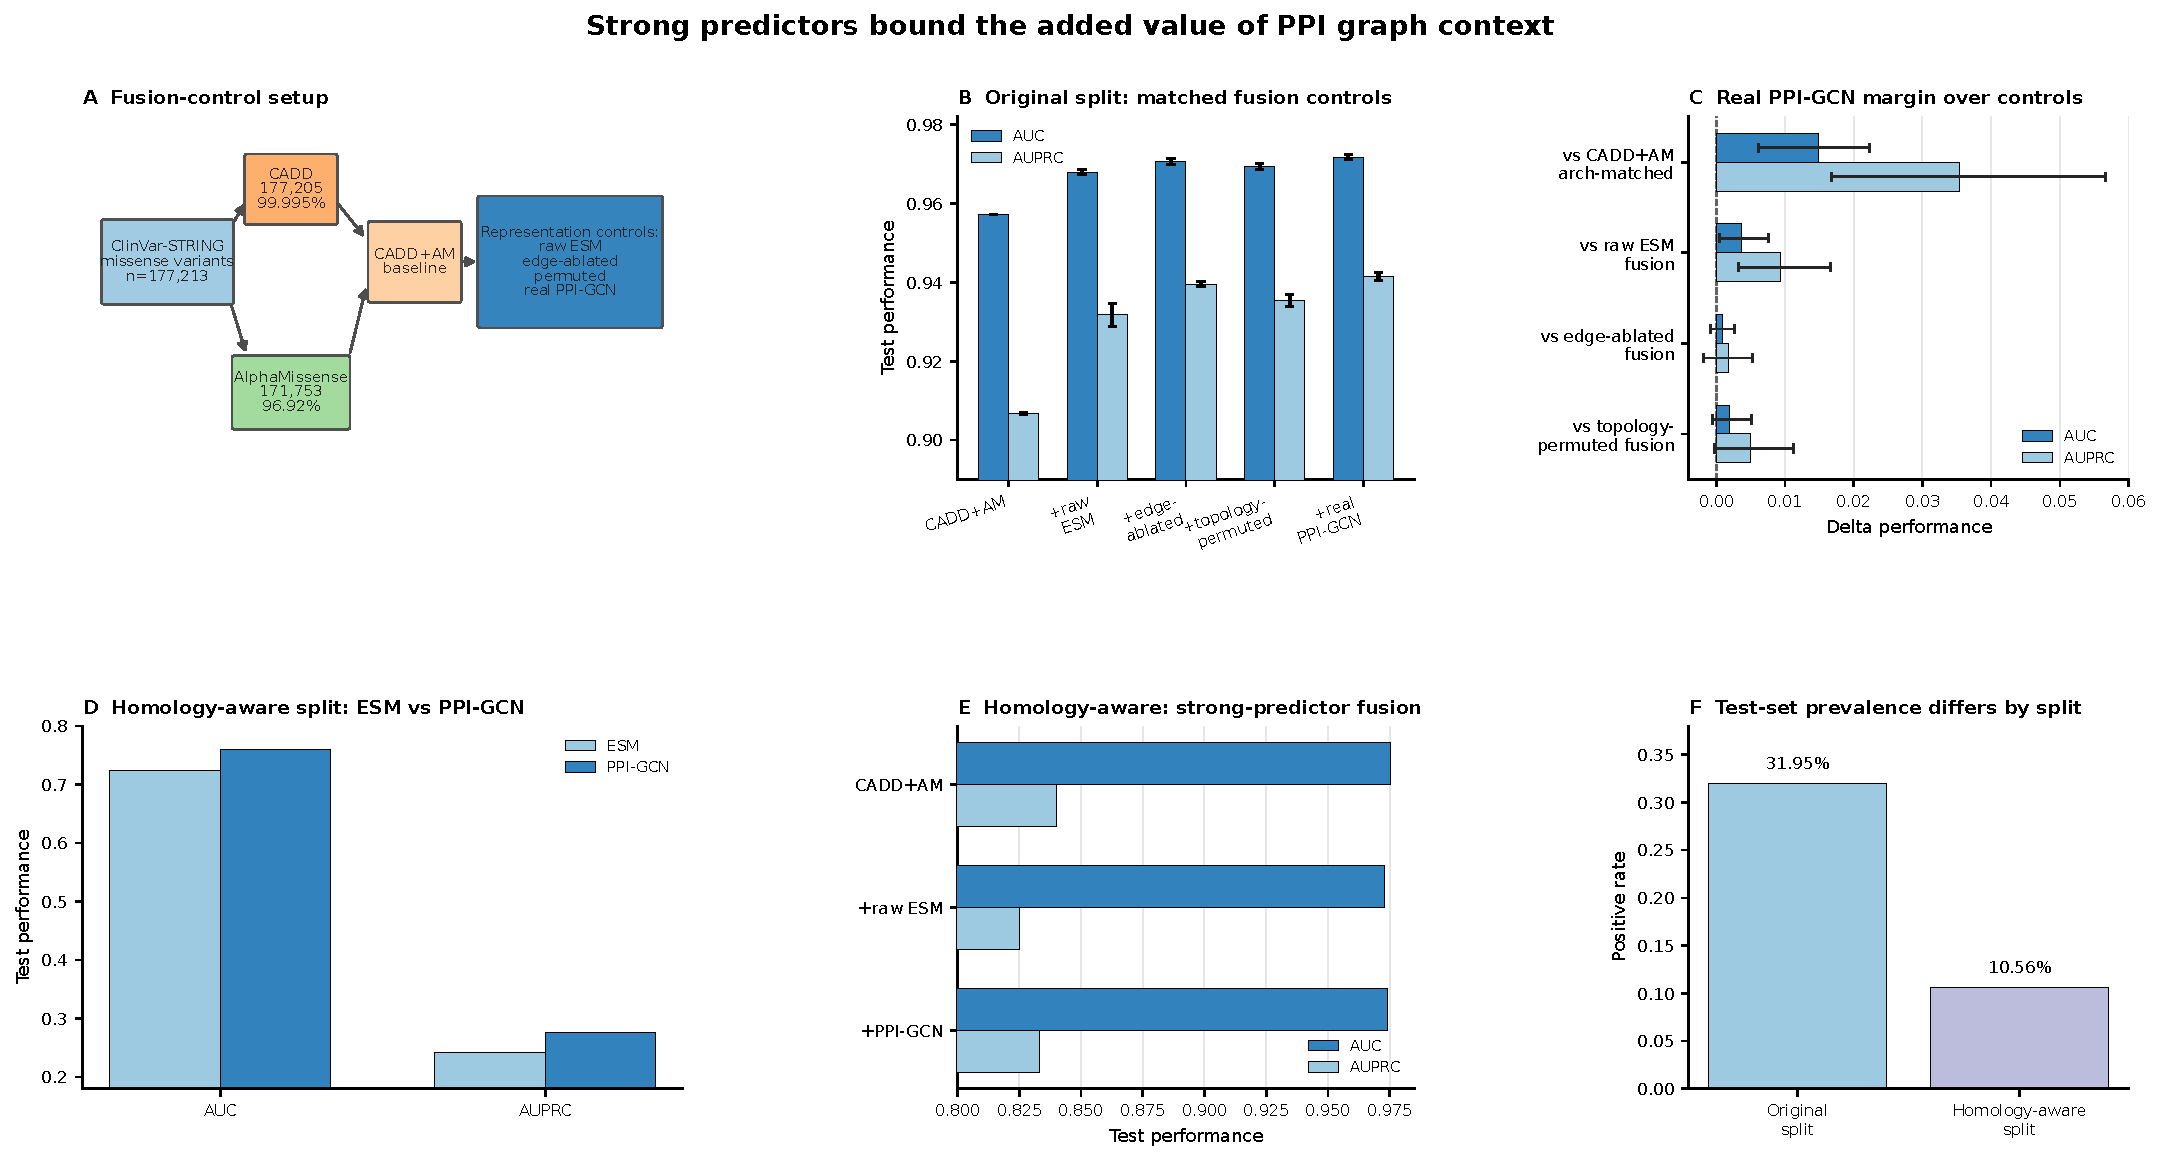
\includegraphics[width=0.98\textwidth]{figure_drafts/Figure2_fusion_homology_v1_accepted.pdf}
\caption{Strong-predictor fusion and homology-aware evaluation. A, Score matching and fusion-control setup; architecture matching refers to hidden layers, not equal input-parameter counts. B, Original-split fusion means and sample SD across three fits per arm, except permutation (three graphs $\times$ three seeds). C, Full-graph fusion differences computed from ensemble-averaged probabilities, with paired protein-bootstrap 95\% intervals conditional on the fitted models and sampled graphs. The point estimates need not equal differences between the mean metrics in B. D, Single-fit homology-aware representation comparison. E, Homology-aware fusion: the score-only and raw-ESM fusion bars show means across three fits, whereas graph fusion shows one fitted-model estimate. Standard deviations for the repeated fits are reported in Supplementary Table 3B. F, Test-set positive prevalence. The ablated/permuted and full encoders differ in self-loop convention.}
\label{fig:fusion_homology}
\end{figure*}

\subsection{Exploratory graph gains across topology contexts}

ESM representation space showed modest correspondence with PPI topology. Sampled PPI-neighbour pairs had mean ESM cosine similarity 0.8789 compared with 0.8639 for random protein pairs, and within-community pairs had higher similarity than between-community pairs (0.8743 versus 0.8642; Fig. 3A). This pattern is consistent with modest correspondence between ESM representation space and PPI network structure before propagation.

Graph-derived gains were not monotonic with simple centrality. Mid-k-core variants showed $\Delta$ AUC +0.0775 and $\Delta$ AUPRC +0.1049, whereas high-degree variants showed $\Delta$ AUC -0.0178 (Fig. 3B). Performance differences also varied across betweenness and clustering strata: low- and mid-betweenness groups showed positive AUC gains (+0.0614 and +0.0522), while high betweenness showed a negative AUC difference (-0.0145); mid- and high-clustering groups showed positive gains, while low clustering was close to zero (Fig. 3C).

Neighbour-risk stratification and joint topology maps showed heterogeneous performance differences. Low-, mid- and high-neighbour-risk strata all had positive AUC gains (+0.0641, +0.0265 and +0.0284), with different AUC and AUPRC profiles across strata (Fig. 3D). Exploratory joint topology maps identified stronger positive and negative profiles, including mid-k-core plus high-betweenness variants ($\Delta$ AUC +0.1429), mid-k-core plus mid-clustering variants (+0.1408), high-neighbour-risk plus mid-k-core variants (+0.1274), and high-k-core plus low-clustering variants (-0.0532; Fig. 3E,F). These profiles were selected after examining 53 joint cells on the same test set. Their variant-level intervals do not account for within-protein dependence, subgroup selection or multiple comparisons, and the findings require independent validation.

\begin{figure*}[!t]
\centering
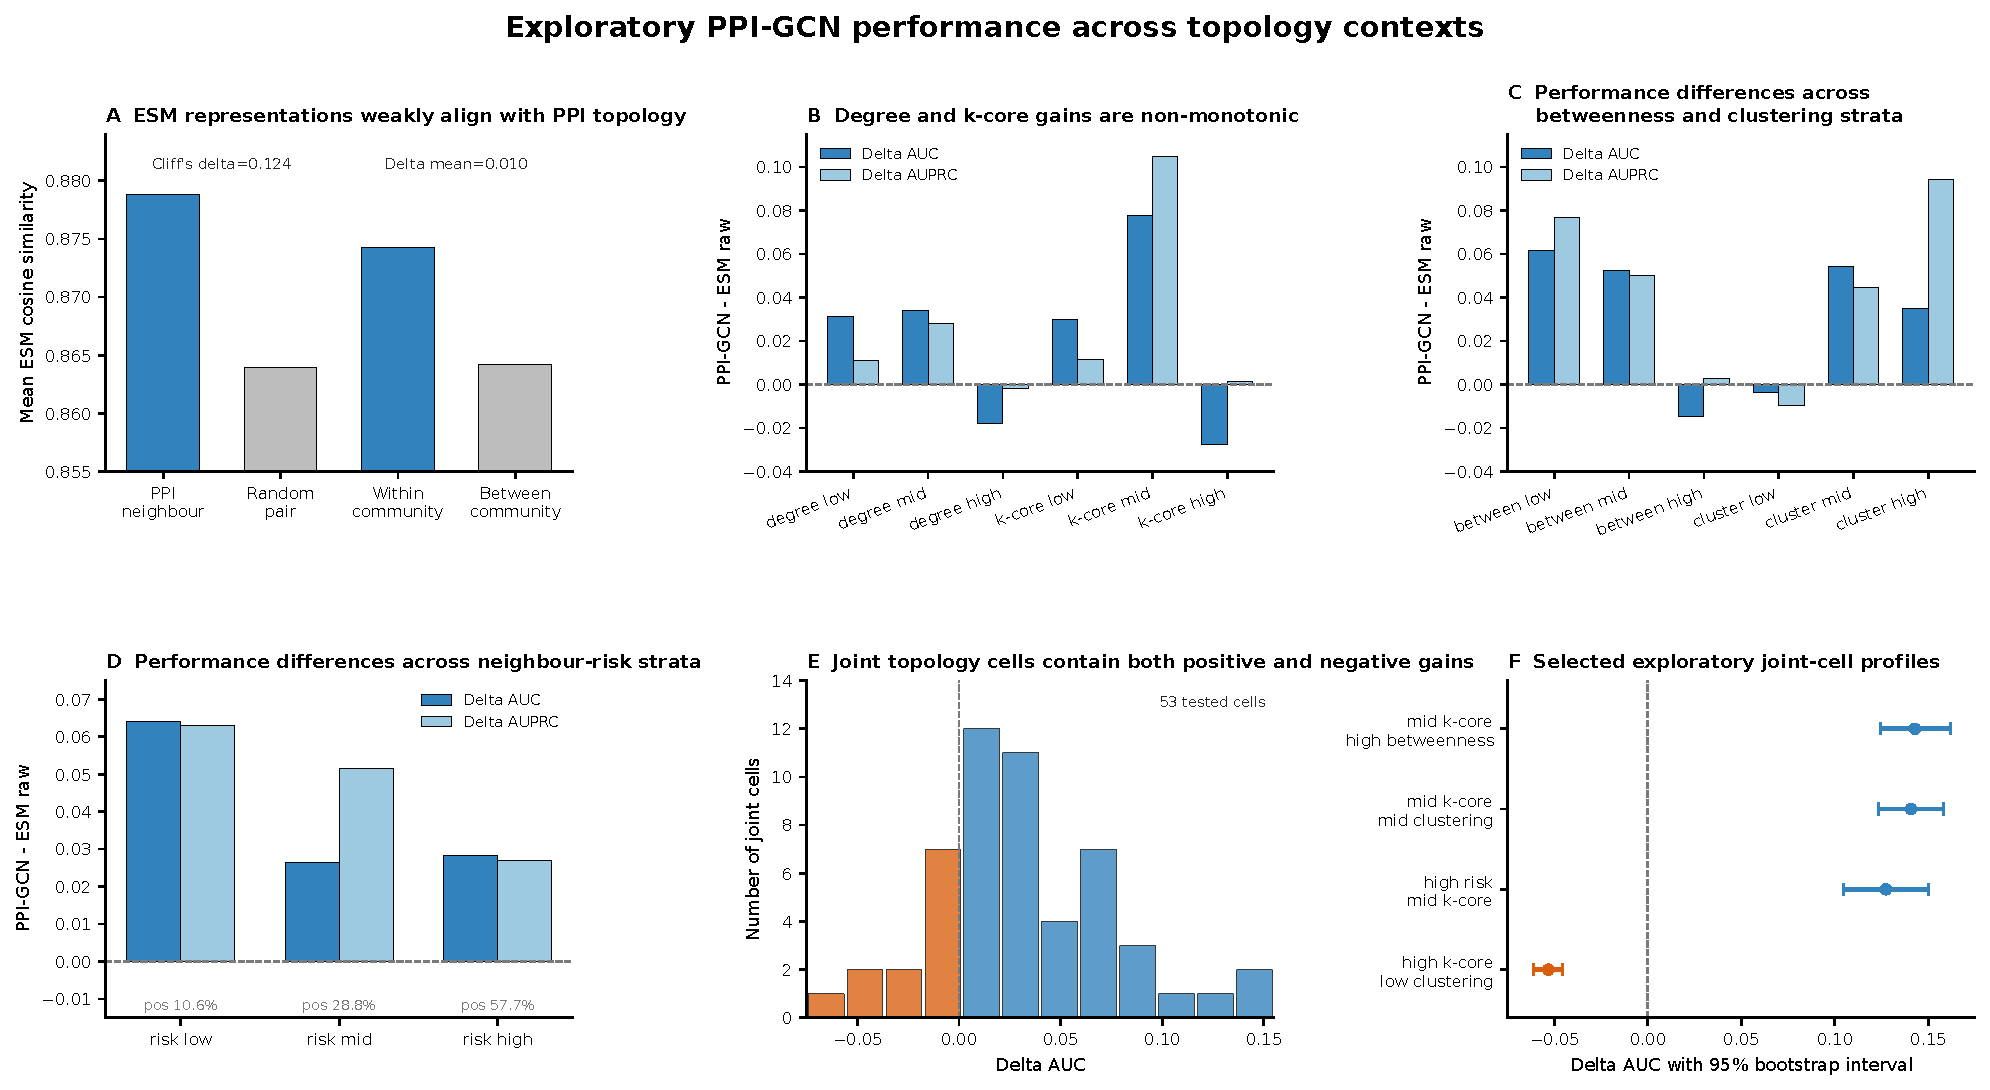
\includegraphics[width=0.98\textwidth]{figure_drafts/Figure3_topology_context_v1_accepted.pdf}
\caption{Exploratory topology-context analysis. A, ESM similarity across network relationships. B--D, Performance differences across network strata. E, AUC differences across 53 joint cells. F, Selected profiles with variant-level bootstrap intervals. B--F use a fixed reference pair. The within-cell variant-bootstrap intervals do not account for within-protein dependence or post-hoc subgroup selection and are not adjusted for multiple comparisons.}
\label{fig:topology_context}
\end{figure*}

\subsection{Graph augmentation reshapes false-negative and false-positive predictions differently}

At a fixed decision-score threshold of 0.5, raw ESM and PPI-GCN were jointly correct for 11,875 test variants and jointly wrong for 3,965 variants. PPI-GCN corrected 1,436 variants and degraded 944 variants relative to raw ESM. Corrected variants included 837 pathogenic false negatives rescued and 599 benign false positives suppressed, whereas degraded variants included 904 benign true negatives converted to false positives and 40 pathogenic true positives converted to false negatives (Fig. 4A).

The retained-reference \CADDAM{} baseline and graph-fusion model were jointly correct for 15,981 variants and jointly wrong for 1,298 variants; graph fusion corrected 666 variants and degraded 275 variants. The corrected set contained more suppressed false positives than rescued false negatives (444 versus 222; Fig. 4B). Figure 4B uses this retained-reference model pair, while Figure 2 reports the architecture-matched repeated-run comparison.

Topology profiles differed between rescued false negatives and suppressed false positives. In the raw ESM to PPI-GCN comparison, rescued false negatives had higher degree, neighbour-risk, neighbour pathogenic rate, neighbour training-variant count and betweenness; suppressed false positives had higher clustering coefficient and within-community neighbour fraction (Fig. 4C). For graph fusion, the degree and neighbour-risk contrasts had the same direction, whereas the clustering-coefficient contrast reversed (Fig. 4D). Figure 4E shows directions of group-mean differences. Figure 4F compares rescued and persistent false negatives within baseline false-negative cases, without continuous prediction-difficulty matching. We interpret these feature contrasts descriptively because variants mapped to the same protein share network features.

\begin{figure*}[!t]
\centering
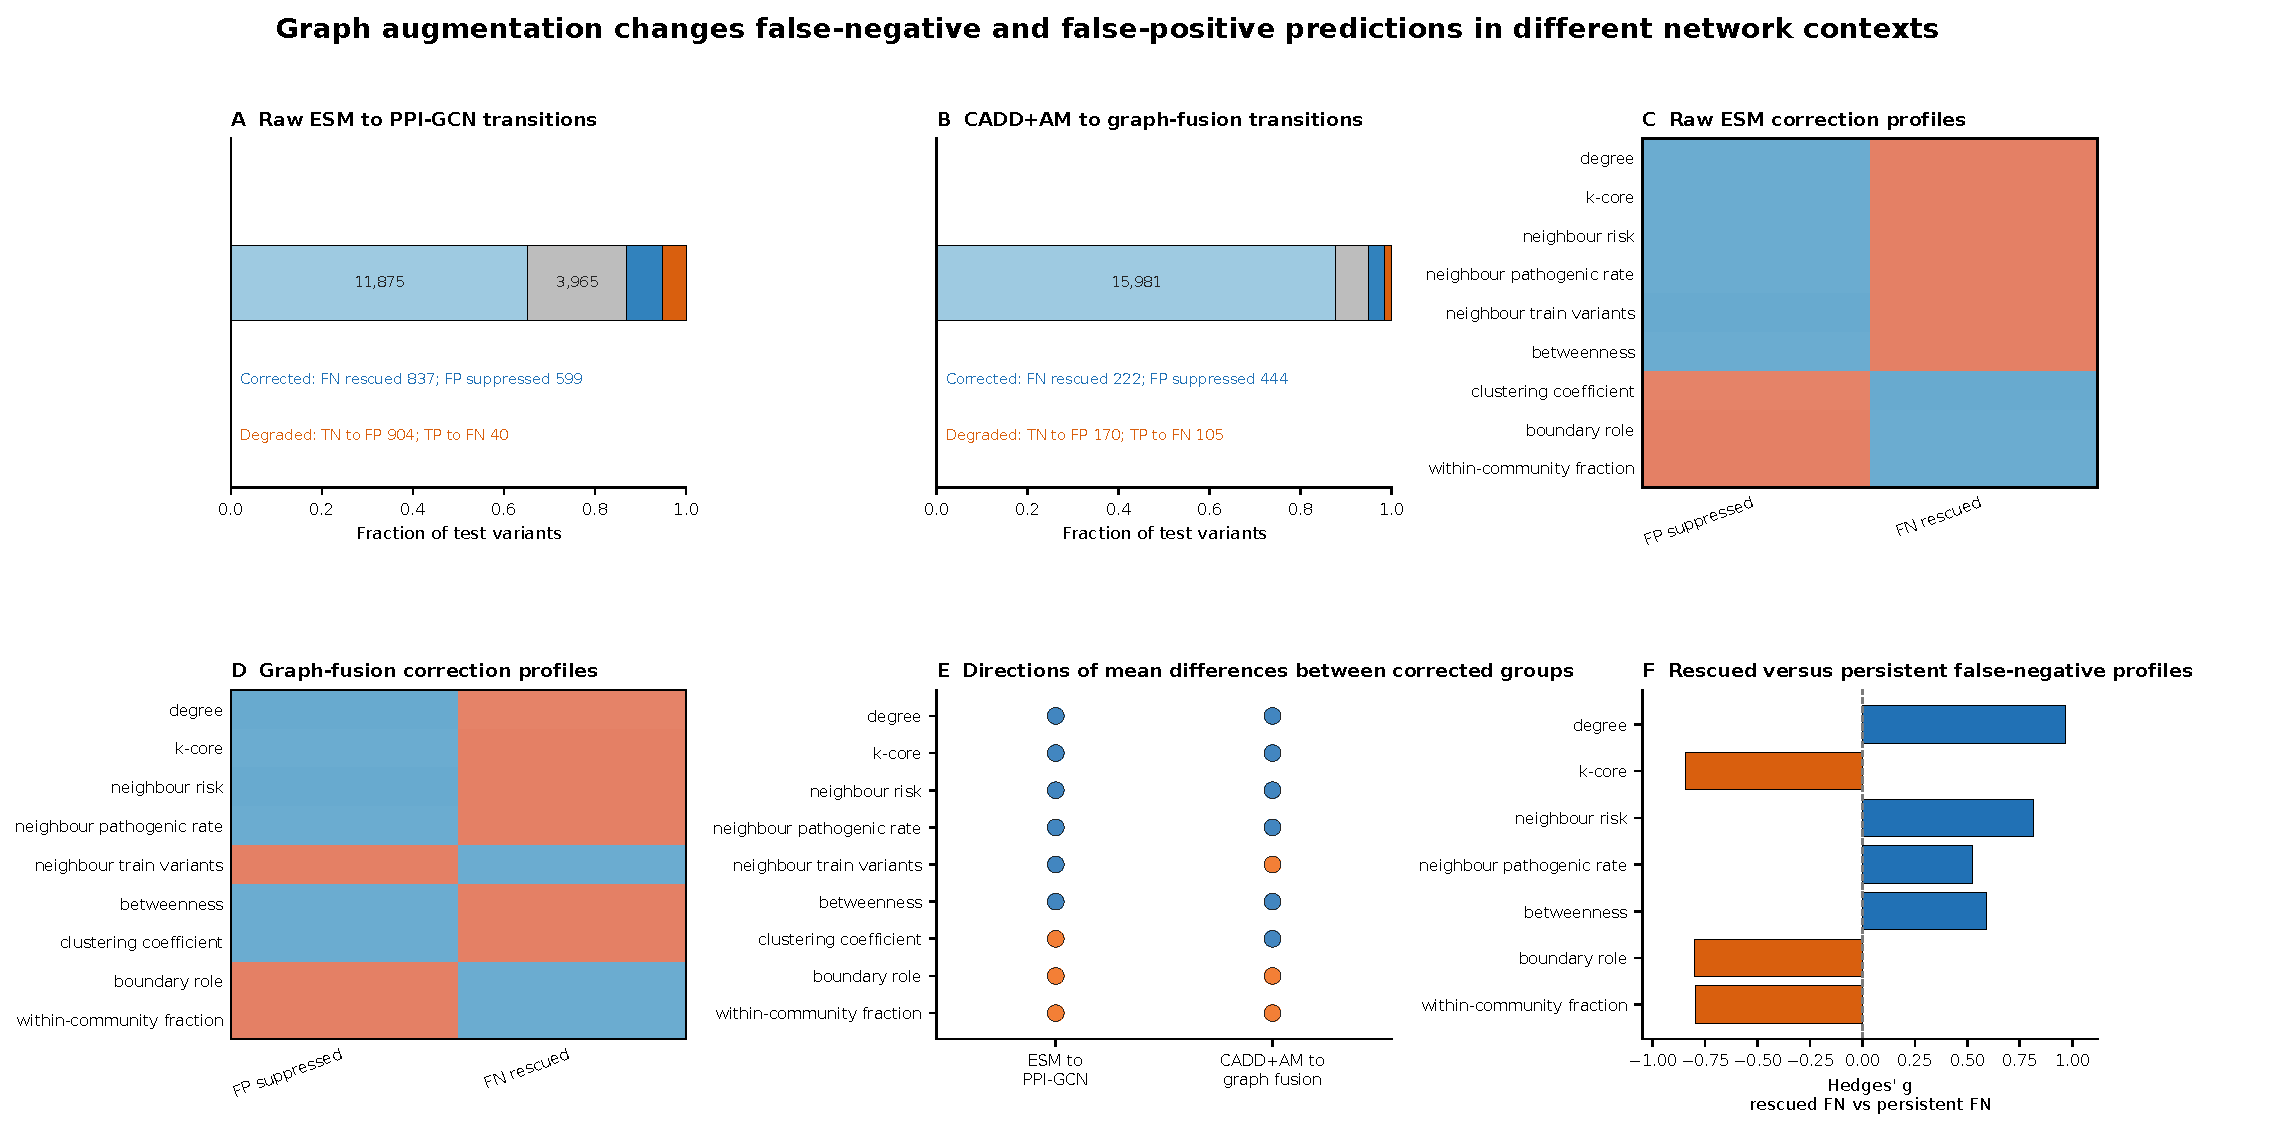
\includegraphics[width=0.98\textwidth]{figure_drafts/Figure4_prediction_transitions_v2_accepted.pdf}
\caption{Prediction transitions and descriptive topology profiles. A--B, Raw ESM to PPI-GCN and score-only to graph-fusion transitions at threshold 0.5, using fixed reference pairs. C--D, Row-centered, range-scaled feature means: warm/blue indicates above/below the row mean. E, Blue/orange indicates higher means in rescued false negatives/suppressed false positives. F, Descriptive Hedges\textquotesingle{} $g$ comparing rescued and persistent false negatives within the raw-ESM baseline false-negative group; blue and orange denote positive and negative effects. Feature comparisons are descriptive and make no inferential significance claims.}
\label{fig:prediction_transitions}
\end{figure*}

\subsection{Second-network validation with BioGRID}

BioGRID did not show a consistent additional benefit over raw-embedding controls (Table~\ref{tab:biogrid}). Under the original split, its fusion improved on scores alone (ensemble $\Delta$AUC +0.0124, protein-bootstrap 95\% CI [+0.0034, +0.0210]), but not clearly on raw-ESM fusion (+0.0009, [-0.0011, +0.0036]). The homology-aware BioGRID fusion estimate was below the score baseline ($\Delta$AUC -0.00204, [-0.00421, -0.00004]). These results limit claims of network-independent gains; complete paired controls and AUPRC intervals are in Supplementary Table 9.

\begin{table}[t]
\caption{BioGRID results under shared training settings.}
\label{tab:biogrid}
\centering\footnotesize\setlength{\tabcolsep}{3pt}
\begin{tabular}{@{}>{\raggedright\arraybackslash}p{0.26\columnwidth}>{\raggedright\arraybackslash}p{0.24\columnwidth}>{\raggedright\arraybackslash}p{0.42\columnwidth}@{}}
\hline
Setting & Mean AUC / AUPRC & Ensemble $\Delta$AUC vs raw [95\% CI] \\
\hline
Original representations & 0.7592 / 0.6043 & -0.0201 [-0.0480, +0.0101] \\
Original fusion & 0.9693 / 0.9344 & +0.0009 [-0.0011, +0.0036] \\
Homology fusion & 0.9730 / 0.8265 & +0.0005 [-0.0008, +0.0017] \\
\hline
\end{tabular}
\par\smallskip\raggedright\footnotesize
Each setting uses three fits per model. Raw denotes raw ESM for representations and raw-ESM fusion for fusion rows. Differences use mean probabilities and paired protein bootstrap within this comparison; SD and all comparator metrics are in Supplementary Table 9.
\end{table}

\section{Discussion}

PPI graph augmentation improved benchmark performance in the shared-graph evaluation, with effects that varied by evaluation design and baseline choice. PPI-GCN improved over raw ESM in the original split, while the graph controls suggested sensitivity to connectivity and topology under differing operator and training settings. With \CADDAM{} included, raw ESM, edge-ablated PPI-GCN and topology-permuted PPI-GCN all produced large fusion gains, while real PPI-GCN was only modestly higher. The strong-predictor fusion gain primarily reflects protein-representation complementarity, with a smaller full-graph margin.

Under the homology-aware split, PPI-GCN remained useful relative to raw ESM. The retained graph-fusion estimate was lower than the repeated-run architecture-matched \CADDAM{} baseline when homologous protein clusters were kept within partitions. Redundant high-dimensional features, extra input-layer parameters, overfitting and feature scaling may explain the limited increment, but were not tested individually. The single graph-fusion fit also limits conclusions about a stable disadvantage. The prevalence shift limits cross-split AUPRC comparison.

Graph propagation changed predictions in heterogeneous topology contexts. These post-hoc associations do not establish correction mechanisms. BioGRID validation further shows that fusion complementarity need not imply a reliable graph-specific increment. STRING and BioGRID differ in density, coverage and evidence types and overlap in interactions, so their comparison does not isolate biological evidence quality. Independent cohorts would be needed to assess transfer beyond the ClinVar benchmark.

The evaluation has several constraints. ClinVar labels may reflect submission bias and future label updates \cite{Landrum2020ClinVar}. Unknown historical overlap with the development data of CADD and AlphaMissense limits prospective interpretation of their benchmark scores. Protein-level mapping omits isoform-specific effects and transcript ambiguity. STRING combined scores integrate several evidence channels and extend beyond direct physical interactions \cite{Szklarczyk2023STRING}. The transductive split and direct-edge ablation retain train-validation, validation-test and higher-order paths. Validation AUC guided checkpoint selection, and the retained PPI-GCN run showed a larger validation gain than test gain; the conclusions draw on held-out test metrics, repeated-seed summaries and protein-clustered uncertainty. The homology-aware prevalence shift limits cross-split AUPRC comparison. Figure 4 transition counts depend on a fixed decision-score threshold, and class-weighted sigmoid outputs are not calibrated clinical probabilities. All fusion controls used identical preprocessing, though alternative feature scaling may change absolute performance. The audit uses retained processed outputs and a compact source-data archive, with provider-controlled resources available from their original sources. The conclusions concern fixed propagation, with only downstream classifiers trained, and should not be generalized to trained graph neural networks.

\noindent\textit{Practical recommendations.} Compare graph features with raw embeddings and strong score baselines; report run configurations and protein-level uncertainty. Treat selected topology groups as hypotheses and check decision thresholds and calibration before clinical use.

\section*{Data and Code Availability}

Supplementary Information, code, compact source data, predictions, protocols and checksums are publicly available at \url{https://github.com/brynn-t02/ppi-graph-missense-audit}. Large third-party resources should be obtained from their original providers.

\section*{Acknowledgment}

OpenAI ChatGPT, OpenAI Codex and Anthropic Claude assisted with literature organization, code development and language editing. The authors take responsibility for study design, experimental execution and verification, code review, interpretation, references and the final manuscript.

\IEEEtriggeratref{25}
\begin{thebibliography}{99}
\bibitem{Kircher2014CADD} M. Kircher et al., ``A general framework for estimating the relative pathogenicity of human genetic variants,'' \emph{Nature Genetics}, vol. 46, pp. 310--315, 2014, doi: 10.1038/ng.2892.
\bibitem{Ioannidis2016REVEL} N. M. Ioannidis et al., ``REVEL: an ensemble method for predicting the pathogenicity of rare missense variants,'' \emph{American Journal of Human Genetics}, vol. 99, pp. 877--885, 2016, doi: 10.1016/j.ajhg.2016.08.016.
\bibitem{Qi2021MVP} H. Qi et al., ``MVP predicts the pathogenicity of missense variants by deep learning,'' \emph{Nature Communications}, vol. 12, p. 510, 2021, doi: 10.1038/s41467-020-20847-0.
\bibitem{Sundaram2018PrimateAI} L. Sundaram et al., ``Predicting the clinical impact of human mutation with deep neural networks,'' \emph{Nature Genetics}, vol. 50, pp. 1161--1170, 2018, doi: 10.1038/s41588-018-0167-z.
\bibitem{Frazer2021EVE} J. Frazer et al., ``Disease variant prediction with deep generative models of evolutionary data,'' \emph{Nature}, vol. 599, pp. 91--95, 2021, doi: 10.1038/s41586-021-04043-8.
\bibitem{Cheng2023AlphaMissense} J. Cheng et al., ``Accurate proteome-wide missense variant effect prediction with AlphaMissense,'' \emph{Science}, vol. 381, eadg7492, 2023, doi: 10.1126/science.adg7492.
\bibitem{Lin2023ESM} Z. Lin et al., ``Evolutionary-scale prediction of atomic-level protein structure with a language model,'' \emph{Science}, vol. 379, pp. 1123--1130, 2023, doi: 10.1126/science.ade2574.
\bibitem{Barabasi2011NetworkMedicine} A.-L. Barabasi, N. Gulbahce, and J. Loscalzo, ``Network medicine: a network-based approach to human disease,'' \emph{Nature Reviews Genetics}, vol. 12, pp. 56--68, 2011, doi: 10.1038/nrg2918.
\bibitem{Menche2015DiseaseModules} J. Menche et al., ``Disease networks. Uncovering disease-disease relationships through the incomplete interactome,'' \emph{Science}, vol. 347, 1257601, 2015, doi: 10.1126/science.1257601.
\bibitem{Sahni2015InteractionPerturbation} N. Sahni et al., ``Widespread macromolecular interaction perturbations in human genetic disorders,'' \emph{Cell}, vol. 161, pp. 647--660, 2015, doi: 10.1016/j.cell.2015.04.013.
\bibitem{Chen2018InteractomePerturbation} S. Chen et al., ``An interactome perturbation framework prioritizes damaging missense mutations for developmental disorders,'' \emph{Nature Genetics}, vol. 50, pp. 1032--1040, 2018, doi: 10.1038/s41588-018-0130-z.
\bibitem{Yates2014SuSPect} C. M. Yates, I. Filippis, L. A. Kelley, and M. J. E. Sternberg, ``SuSPect: enhanced prediction of single amino acid variant phenotype using network features,'' \emph{Journal of Molecular Biology}, vol. 426, pp. 2692--2701, 2014, doi: 10.1016/j.jmb.2014.04.026.
\bibitem{Ozturk2022NetworkFeatures} K. Ozturk and H. Carter, ``Predicting functional consequences of mutations using molecular interaction network features,'' \emph{Human Genetics}, vol. 141, pp. 1195--1210, 2022, doi: 10.1007/s00439-021-02329-5.
\bibitem{Zhang2022gMVP} H. Zhang, M. S. Xu, X. Fan, W. K. Chung, and Y. Shen, ``Predicting functional effect of missense variants using graph attention neural networks,'' \emph{Nature Machine Intelligence}, vol. 4, no. 11, pp. 1017--1028, 2022, doi: 10.1038/s42256-022-00561-w.
\bibitem{Cheng2021VEGN} J. Cheng, C. Lawrence, and M. Niepert, ``VEGN: variant effect prediction with graph neural networks,'' arXiv:2106.13642, 2021, doi: 10.48550/arXiv.2106.13642.
\bibitem{Yu2025GNNMAP} H. Yu et al., ``A graph neural network approach for accurate prediction of pathogenicity in multi-type variants,'' \emph{Briefings in Bioinformatics}, vol. 26, bbaf151, 2025, doi: 10.1093/bib/bbaf151.
\bibitem{Ghadie2025DiseaseSpecificGNN} M. Ghadie, S. Sardaar, and Y. Trakadis, ``Disease-specific prediction of missense variant pathogenicity with DNA language models and graph neural networks,'' \emph{Bioengineering}, vol. 12, p. 1098, 2025, doi: 10.3390/bioengineering12101098.
\bibitem{Littmann2022ProteinMLTips} Q. Hou, K. Waury, D. Gogishvili, and K. A. Feenstra, ``Ten quick tips for sequence-based prediction of protein properties using machine learning,'' \emph{PLOS Computational Biology}, vol. 18, no. 12, Art. no. e1010669, 2022, doi: 10.1371/journal.pcbi.1010669.
\bibitem{Teufel2023GraphPart} F. Teufel, M. H. Gislason, J. J. Almagro Armenteros, A. R. Johansen, O. Winther, and H. Nielsen, ``GraphPart: homology partitioning for biological sequence analysis,'' \emph{NAR Genomics and Bioinformatics}, vol. 5, lqad088, 2023, doi: 10.1093/nargab/lqad088.
\bibitem{Landrum2020ClinVar} M. J. Landrum et al., ``ClinVar: improvements to accessing data,'' \emph{Nucleic Acids Research}, vol. 48, pp. D835--D844, 2020, doi: 10.1093/nar/gkz972.
\bibitem{Szklarczyk2023STRING} D. Szklarczyk et al., ``The STRING database in 2023: protein-protein association networks and functional enrichment analyses for any sequenced genome of interest,'' \emph{Nucleic Acids Research}, vol. 51, pp. D638--D646, 2023, doi: 10.1093/nar/gkac1000.
\bibitem{Kipf2017GCN} T. N. Kipf and M. Welling, ``Semi-supervised classification with graph convolutional networks,'' \emph{International Conference on Learning Representations}, 2017.
\bibitem{Steinegger2017MMseqs2} M. Steinegger and J. Soding, ``MMseqs2 enables sensitive protein sequence searching for the analysis of massive data sets,'' \emph{Nature Biotechnology}, vol. 35, pp. 1026--1028, 2017, doi: 10.1038/nbt.3988.
\bibitem{Kingma2015Adam} D. P. Kingma and J. Ba, ``Adam: a method for stochastic optimization,'' \emph{International Conference on Learning Representations}, 2015, arXiv:1412.6980.
\bibitem{Schubach2024CADDv17} M. Schubach et al., ``CADD v1.7: using protein language models, regulatory CNNs and other nucleotide-level scores to improve genome-wide variant predictions,'' \emph{Nucleic Acids Research}, vol. 52, no. D1, pp. D1143--D1154, 2024, doi: 10.1093/nar/gkad989.
\bibitem{Efron1993Bootstrap} B. Efron and R. J. Tibshirani, \emph{An Introduction to the Bootstrap}. Chapman \& Hall/CRC, 1993.
\bibitem{Benjamini1995FDR} Y. Benjamini and Y. Hochberg, ``Controlling the false discovery rate: a practical and powerful approach to multiple testing,'' \emph{Journal of the Royal Statistical Society: Series B}, vol. 57, pp. 289--300, 1995, doi: 10.1111/j.2517-6161.1995.tb02031.x.
\bibitem{Saito2015PrecisionRecall} T. Saito and M. Rehmsmeier, ``The precision-recall plot is more informative than the ROC plot when evaluating binary classifiers on imbalanced datasets,'' \emph{PLOS ONE}, vol. 10, e0118432, 2015, doi: 10.1371/journal.pone.0118432.
\bibitem{Stark2006BioGRID} C. Stark, B.-J. Breitkreutz, T. Reguly, L. Boucher, A. Breitkreutz, and M. Tyers, ``BioGRID: a general repository for interaction datasets,'' \emph{Nucleic Acids Research}, vol. 34, pp. D535--D539, 2006, doi: 10.1093/nar/gkj109.
\end{thebibliography}
\end{document}
